\documentclass{standalone}

\usepackage{tikz}

\begin{document}
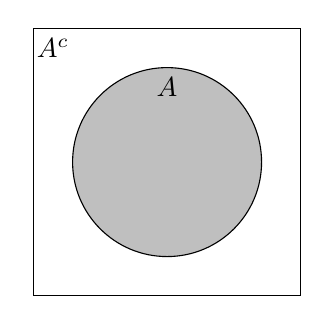
\begin{tikzpicture}
    \path[fill=lightgray]
        (0,0)circle[radius=1.2cm]
    ;
    \path[draw]
        (0,0) circle [radius=1.2cm]
    ;
    \node at (0, 0.95) {$A$};
    \node at (-1.45, 1.45) {$A^c$};
    \draw (-1.7, -1.7) rectangle (1.7, 1.7);
\end{tikzpicture}
\hspace{1cm}
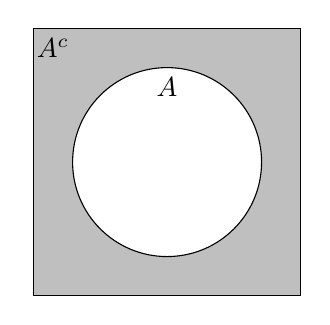
\begin{tikzpicture}
    \path[fill=lightgray,even odd rule]
        (-1.7, -1.7) rectangle (1.7, 1.7)
        (0,0)circle[radius=1.2cm]
    ;
    \path[draw]
        (0,0) circle [radius=1.2cm]
    ;
    \node at (0, 0.95) {$A$};
    \node at (-1.45, 1.45) {$A^c$};
    \draw (-1.7, -1.7) rectangle (1.7, 1.7);
\end{tikzpicture}
\end{document}
